%%%%%%%%%%%%%%%%%%%%%%%%%%%%%%%%%%%%%%%%%
% Arsclassica Article
% LaTeX Template
% Version 1.1 (1/8/17)
%
% This template has been downloaded from:
% http://www.LaTeXTemplates.com
%
% Original author:
% Lorenzo Pantieri (http://www.lorenzopantieri.net) with extensive modifications by:
% Vel (vel@latextemplates.com)
%
% License:
% CC BY-NC-SA 3.0 (http://creativecommons.org/licenses/by-nc-sa/3.0/)
%
%%%%%%%%%%%%%%%%%%%%%%%%%%%%%%%%%%%%%%%%%

%----------------------------------------------------------------------------------------
%	PACKAGES AND OTHER DOCUMENT CONFIGURATIONS
%----------------------------------------------------------------------------------------

\documentclass[
12pt, % Main document font size
a4paper, % Paper type, use 'letterpaper' for US Letter paper
oneside, % One page layout (no page indentation)
%twoside, % Two page layout (page indentation for binding and different headers)
headinclude,footinclude, % Extra spacing for the header and footer
BCOR5mm, % Binding correction
]{scrartcl}

%%%%%%%%%%%%%%%%%%%%%%%%%%%%%%%%%%%%%%%%%
% Arsclassica Article
% Structure Specification File
%
% This file has been downloaded from:
% http://www.LaTeXTemplates.com
%
% Original author:
% Lorenzo Pantieri (http://www.lorenzopantieri.net) with extensive modifications by:
% Vel (vel@latextemplates.com)
%
% License:
% CC BY-NC-SA 3.0 (http://creativecommons.org/licenses/by-nc-sa/3.0/)
%
%%%%%%%%%%%%%%%%%%%%%%%%%%%%%%%%%%%%%%%%%

%----------------------------------------------------------------------------------------
%	REQUIRED PACKAGES
%----------------------------------------------------------------------------------------

\usepackage[
nochapters, % Turn off chapters since this is an article        
beramono, % Use the Bera Mono font for monospaced text (\texttt)
eulermath,% Use the Euler font for mathematics
pdfspacing, % Makes use of pdftex’ letter spacing capabilities via the microtype package
dottedtoc % Dotted lines leading to the page numbers in the table of contents
]{classicthesis} % The layout is based on the Classic Thesis style

\usepackage{arsclassica} % Modifies the Classic Thesis package

\usepackage[T1]{fontenc} % Use 8-bit encoding that has 256 glyphs

\usepackage[utf8]{inputenc} % Required for including letters with accents

\usepackage{dirtytalk} %for easy quotations just use \say{quotation}

\usepackage{graphicx} % Required for including images
\graphicspath{{Figures/}} % Set the default folder for images

\usepackage{enumitem} % Required for manipulating the whitespace between and within lists

\usepackage{lipsum} % Used for inserting dummy 'Lorem ipsum' text into the template

\usepackage{subfig} % Required for creating figures with multiple parts (subfigures)

\usepackage{amsmath,amssymb,amsthm} % For including math equations, theorems, symbols, etc

\usepackage{varioref} % More descriptive referencing

%----------------------------------------------------------------------------------------
%	THEOREM STYLES
%---------------------------------------------------------------------------------------

\theoremstyle{definition} % Define theorem styles here based on the definition style (used for definitions and examples)
\newtheorem{definition}{Definition}

\theoremstyle{plain} % Define theorem styles here based on the plain style (used for theorems, lemmas, propositions)
\newtheorem{theorem}{Theorem}

\theoremstyle{remark} % Define theorem styles here based on the remark style (used for remarks and notes)

%----------------------------------------------------------------------------------------
%	HYPERLINKS
%---------------------------------------------------------------------------------------

\hypersetup{
%draft, % Uncomment to remove all links (useful for printing in black and white)
colorlinks=true, breaklinks=true, bookmarks=true,bookmarksnumbered,
urlcolor=webbrown, linkcolor=RoyalBlue, citecolor=webgreen, % Link colors
pdftitle={}, % PDF title
pdfauthor={\textcopyright}, % PDF Author
pdfsubject={}, % PDF Subject
pdfkeywords={}, % PDF Keywords
pdfcreator={pdfLaTeX}, % PDF Creator
pdfproducer={LaTeX with hyperref and ClassicThesis} % PDF producer
} % Include the structure.tex file which specified the document structure and layout

\hyphenation{Fortran hy-phen-ation} % Specify custom hyphenation points in words with dashes where you would like hyphenation to occur, or alternatively, don't put any dashes in a word to stop hyphenation altogether

%----------------------------------------------------------------------------------------
%	TITLE AND AUTHOR(S)
%----------------------------------------------------------------------------------------

\title{\normalfont\spacedallcaps{The Explosion of Ariane 5}} % The article title

%\subtitle{Subtitle} % Uncomment to display a subtitle

\author{\spacedlowsmallcaps{André Santos\textsuperscript{1}, Manuel Moreira\textsuperscript{2}, Ricardo Ferreira\textsuperscript{3} }} % The article author(s) - author affiliations need to be specified in the AUTHOR AFFILIATIONS block

\date{October 2018} % An optional date to appear under the author(s)

%----------------------------------------------------------------------------------------

\begin{document}

%----------------------------------------------------------------------------------------
%	HEADERS
%----------------------------------------------------------------------------------------

\renewcommand{\sectionmark}[1]{\markright{\spacedlowsmallcaps{#1}}} % The header for all pages (oneside) or for even pages (twoside)
%\renewcommand{\subsectionmark}[1]{\markright{\thesubsection~#1}} % Uncomment when using the twoside option - this modifies the header on odd pages
\lehead{\mbox{\llap{\small\thepage\kern1em\color{halfgray} \vline}\color{halfgray}\hspace{0.5em}\rightmark\hfil}} % The header style

\pagestyle{scrheadings} % Enable the headers specified in this block

%----------------------------------------------------------------------------------------
%	TABLE OF CONTENTS & LISTS OF FIGURES AND TABLES
%----------------------------------------------------------------------------------------

\maketitle % Print the title/author/date block

\setcounter{tocdepth}{2} % Set the depth of the table of contents to show sections and subsections only

\tableofcontents % Print the table of contents

\listoffigures % Print the list of figures

%\listoftables % Print the list of tables

%----------------------------------------------------------------------------------------
%	ABSTRACT
%----------------------------------------------------------------------------------------

\section*{Abstract} % This section will not appear in the table of contents due to the star (\section*)

On June 4, 1996 an unmanned Ariane 5 rocket launched by the European Space Agency exploded just forty seconds after its lift-off from Kourou, French Guiana. The rocket was on its first voyage, after a decade of development costing \$7 billion. The destroyed rocket and its cargo were valued at \$500 million. A board of inquiry investigated the causes of the explosion and in two weeks issued a report. It turned out that the cause of the failure was a software error in the inertial reference system. Specifically a 64 bit floating point number relating to the horizontal velocity of the rocket with respect to the platform was converted to a 16 bit signed integer. The number was larger than 32,767, the largest integer storeable in a 16 bit signed integer, and thus the conversion failed.

%\lipsum[1] % Dummy text

%----------------------------------------------------------------------------------------
%	AUTHOR AFFILIATIONS
%----------------------------------------------------------------------------------------

%\let\thefootnote\relax\footnotetext{* \textit{up200305418, Faculdade de Engenharia, Universidade do Porto}}

\let\thefootnote\relax\footnotetext{\textsuperscript{1} \textit{up, Faculdade de Engenharia, Universidade do Porto}}
\let\thefootnote\relax\footnotetext{\textsuperscript{2} \textit{up, Faculdade de Engenharia, Universidade do Porto}}
\let\thefootnote\relax\footnotetext{\textsuperscript{3} \textit{up200305418, Faculdade de Engenharia, Universidade do Porto}}

%----------------------------------------------------------------------------------------

\newpage % Start the article content on the second page, remove this if you have a longer abstract that goes onto the second page

%----------------------------------------------------------------------------------------
%	INTRODUCTION
%----------------------------------------------------------------------------------------

\section{Introduction}

The European Space Agency worked for 10 years to produce a rocket capable of launch, into orbit, two satellites weighing more than three tones each. These satellites would give Europe a big advantage and control over the commercial space agency. 

On June 4, 1996, everything was ready at Kourou, French Guiana. The rocket, known has Ariane 5, was launched and just forty seconds after lift-off, exploded.
The destroyed rocket and its cargo were valued in \$500 million and the entire operation costs \$7 billion dollar's.

Thirty seven seconds after ignition, Ariane 5 completely losses guidance and altitude information, due to specification and design error of the inertial reference software system. At 4km of altitude the self-destruction mechanism was triggered, because aerodynamic forces were ripping off parts of the rocket. Consequence of an abrupt course correction, that was not needed, compensating for a wrong turn that had not taken place. Steering was controlled by the on-board computer, which mistakenly thought the rocket needed a course change because of numbers coming from the inertial guidance system. The number was too big and caused an overflow.

When the guidance system shut down, it passed control to an identical, redundant unit, which was running the same software, and the same error occurred again, resulting in the explosion of Ariane 5.

\begin{figure}[tb]
	\centering 
	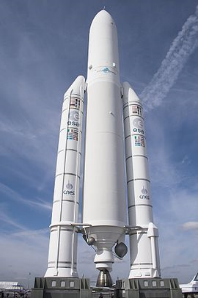
\includegraphics[width=0.5\columnwidth]{ariane5} 
	\caption[The Ariane 5 rocket]{The Ariane 5 rocket, before ignition \cite{hownottocode:2016}} % The text in the square bracket is the caption for the list of figures while the text in the curly brackets is the figure caption
	\label{fig:arianefive} 
\end{figure}

 
%----------------------------------------------------------------------------------------
%	The Failure
%----------------------------------------------------------------------------------------

\section{The Failure}


The rocket steering was controlled by a system, the Inertial Software System (SRI), that uses gyroscopes and accelerometers and sends data to the onboard computer. This software was continuously reading and calculating velocities and angles to correct the course of the rocket, sending information to the steering system.

In order to improve reliability there were a considerable redundancy at  equipment level. Two SRIs operating in parallel, with identical  hardware and software. If the active SRI fails, it immediately switches to the other one. The same was true for other Flight Control Units.

After thirty seven seconds of flight, the Inertial Software System sent an abrupt course correction to the steering system. Though, this correction was not needed, the Inertial Software System thought the rocket had mad a wrong  turn that had not taken place. 

This abrupt turn, created an unexpected pressure on some components of the engine and the rocket started to disintegrate, which triggered the self-destruct mechanism.

Everything was triggered by a conversion of a 64-bit number into a 16-bit number which caused an overflow and the shut down of the Inertial Software System. When this happened, the control was passed to the backup software, but this one also tried the same conversion, they were running the same  software, and a chain of events occurred ending in the self destruction of Ariane 5.

Professor J. L. Lions, in charge of the analysis of the problem, in it's report \cite{Report:1996} stated that the failure was:

\say{The internal SRI software exception was caused during execution of a data conversion from 64-bit floating point to 16-bit signed integer value. The floating point number which was converted had a value greater than what could be represented by a 16-bit signed integer.}

\begin{figure}[tb]
	\centering 
	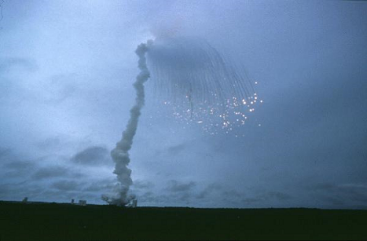
\includegraphics[width=0.5\columnwidth]{ariane5-explosion} 
	\caption[The Ariane 5 Explosion]{The Ariane 5 explosion after a few seconds of ignition \cite{hownottocode:2016}} % The text in the square bracket is the caption for the list of figures while the text in the curly brackets is the figure caption
	\label{fig:arianeexplosion} 
\end{figure}

%------------------------------------------------

\subsection{How it happens}

The On-Board Computer (OBC) commands the nozzles on base of data transmitted by the active Inertial Reference System (SRI). When the OBC asked flight  information to the SRI, the data received did not contain proper information,  but showed a diagnostic bit pattern of the computer running the SRI. This data was interpreted has flight data. 

The OBC was not expecting bad data since a fall back system was in place, but both SRI's have failed due to a software exception.

The software exception was caused during execution of a data conversion from 64-bit floating point to 16-bit signed integer value. The floating point number which was converted had a value greater than what could be represented by a 16-bit signed integer. This resulted in an Operand Error. The data conversion instructions were not protected from causing an Operand Error, although other conversions of comparable variables in the same place in the code were protected.

The curious part is that this part of the software only computes meaningful results before lift-off, as soon has the launcher starts, the function serves no purpose. But, the function continues to calculate data for 40 seconds after lift-off. This time sequence was a requirement of the previous rocket, Ariane 4, and not a requirement of Ariane 5.

This happened only by a wrong design implementation and not well specified requirements.

\begin{figure}[tb]
	\centering 
	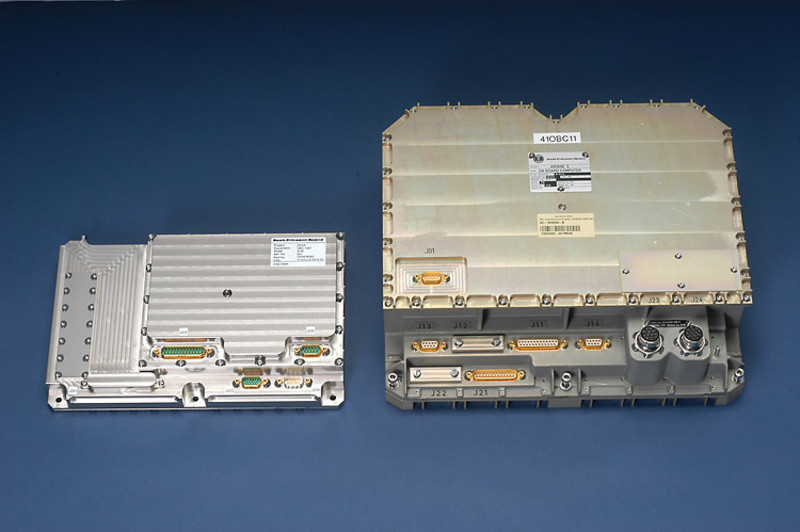
\includegraphics[width=0.5\columnwidth]{onboardComputers} 
	\caption[The On Board computers]{The On Board computers were the faulty software was running \cite{hownottocode:2016}} % The text in the square bracket is the caption for the list of figures while the text in the curly brackets is the figure caption
	\label{fig:onboardcomputers} 
\end{figure}

%------------------------------------------------

\subsection{An overflow in programming and how to prevent it}

An overflow in programming \cite{integeroverflow:wikipedia} occurs when an arithmetic operation attempts to  create a numeric value that is outside of the range that can be represented with a given number of digits, either larger than the maximum or lower than the minimum representable value.

An overflow can lead to unintended behaviour and compromise a program's reliability.

Like said on the previous section, on Ariane 5 the software was trying to convert a 64-bit floating point number to a 16-bit signed integer.

This type of conversions on Ariane 5 were not foreseen, but simple approaches could be used to avoid this software exception. Furthermore, overflow can always be avoid. 

Some of the methods are:

\begin{itemize}[noitemsep] % [noitemsep] removes whitespace between the items for a compact look
	\item Allocating variables with data types large enough to contain all values that may be computed or stored in them
	\item Using tests or software routines to handling exceptions and do different processing to mitigate the overflow.
	\item Using flags in the code to propagate the error and void the calculation at the end
\end{itemize}

%------------------------------------------------

\subsection{The Programming language used}

The software was written in Ada, a programming language extended from Pascal\cite{ada:wikipedia}.

Ada was named after Ada Lovelace\textsuperscript{a}, considered the first computer programmer and is a language well suited for embedded systems, real time applications, numerical and financial systems and object-oriented programming. 

The language has built-in support for design by contract. This means that software designers can define conditions and specifications (contracts) related with the functions and it's results, giving an extra layer of reliability to the code. This does not replace unit testing, integration testing and system testing, rather complements it with internal self tests. 

Features of Ada include: strong typing, modularity mechanisms (packages), run-time checking, parallel processing (tasks, synchronous message passing, protected objects, and nondeterministic select statements), exception handling, and generics.

Some say that the Ada language does not provide good exception handling and that was the origin of the problem. But that wasn't the true \cite{programingProblem:PeterB}, neither the cause of the problem. Ada has everything to avoid error. The problem was on a poor requirements description and analyses and not using the full potential of the language.

The same conclusion was written on the report of the incident\cite{Report:1996}:

\say{The failure of the Ariane 501 was caused by the complete loss of guidance and altitude information 37 seconds after start of the main engine ignition sequence (30 seconds after lift-off). This loss of information was due to specification and design errors in the software of the inertial reference system.}
\say{Not all the conversions were protected because... To determine the vulnerability of unprotected code, an analysis was performed on every operation which could give rise to an ... operand error. This led to protection being added to four of seven variables... in the Ada code. However, three of the variables were left unprotected.}

\let\thefootnote\relax\footnotetext{\textsuperscript{a} \textit{\url{https://en.wikipedia.org/wiki/Ada_Lovelace}}}

% -----------------------------------------------

\subsection{Lack of Software Engineering guidelines}

ESA\textsuperscript{b} did not prosecute the team of engineers that develop the SRI software, but the board that analysed the disaster found some ethical and methodologies issues.

In a project like this, engineering methods should have been used \cite{softwaretechniques:1970}, but they were totally neglected. The software development should had follow the following topics:
\begin{itemize}[noitemsep] % [noitemsep] removes whitespace between the items for a compact look
	\item Design
	\item Documentation
	\item Testing
	\item Review
\end{itemize}

The team of engineers involved should also had a more ethical approach with the project by:

\begin{itemize}[noitemsep] % [noitemsep] removes whitespace between the items for a compact look
	\item Exposing risks openly to supervisors
	\item Ensuring that their products meet highest professional standards
	\item Exposing their knowledge to others
\end{itemize}

All the protocol was neglected which lead to erroneous software and bad engineering practices, which ended in bad software, that is:

\begin{itemize}[noitemsep] % [noitemsep] removes whitespace between the items for a compact look
	\item Hard to maintain
	\item Very expensive
	\item Without remote access
	\item Without error handling
	\item Without a proper test suit
\end{itemize}

Like other disciples, Software engineering \cite{softwaretechniques:1970}, has at its disposal methods for proper creation of software to ensure software quality and flexibility. The Ariane 5 event was a warning to the engineering community and that this methodologies and techniques are not only academic. The Inquiry Board \cite{Report:1996} mad a number of recommendations to improve the quality of software like:

\say{Give the justification documents the same attention as code. Improve the technique for keeping code and its justifications consistent.}

\say{Review the test coverage of existing equipment and extend it where it is deemed necessary.}

\say{Wherever technically feasible, consider confining exceptions to tasks and devise backup capabilities.}

\say{Prepare a test facility including as much real equipment as technically feasible, inject realistic input data, and perform complete, closed-loop, system testing. Complete simulations must take place before any mission. A high test coverage has to be obtained.}

More recommendations can be found at the report.

\let\thefootnote\relax\footnotetext{\textsuperscript{a} \textit{European Space Agency}}

%----------------------------------------------------------------------------------------
%	Losses and Impacts
%----------------------------------------------------------------------------------------

\section{Losses and Impacts}

The European Space Agency, ended up spending 7 billion dollar's and it's reputation.

Ariane 5 was part of the Ariane family of rockets, created to deliver satellites to the earth orbit. With this program ESA was trying to achieve commercial control on the area of satellites, but ended up loosing the rocket mechanism, revenue and market share. ESA lost the European faith on the program.

The project had some stack holders like European Space Agency, Centre Nationel de d'Etudes Spatial, governments, european taxpayers, european shareholders, and all of them lost money with this software bug, France alone lost 3 billion dollars.

After an extensive investigation, nobody was found liable and there was no one to blame, only faulty software. At the time of the event, pursuing the team of developers would have been even more disastrous and would ended up in loss of clients and loss of trust in the program.

This event attracted the attention of the public, politicians and the head of organizations to the high risk of bad practices in complex computational systems, which increased investment in research \cite{lessonsofAriane:Jean}.


%----------------------------------------------------------------------------------------
%	Losses and Impacts
%----------------------------------------------------------------------------------------

\section{Conclusion}

The defect on the Ariane 5 was the result of several factors, but the most significant was neglecting software engineering guidelines. The software didn't had proper exception handling neither a good test scenario. Furthermore, the part of the software that caused the bug was a requirement of the former Ariane 4 and of no use in Ariane 5. This shows that besides bad practices in development the team had also fail to specify the requirements for the project.

Despite all the financial losses, the Ariane 5 explosion, brought to attention of the public the high risk of bad practices in software development, specially if we are talking about life critical systems. This increased the investment in research and now, design by contract\cite{designByContract:wikipedia} and other design techniques and guidelines are well documented and used in a large variety of projects.

This event was carefully investigated by an independent inquiry board which produced a report with valuable information about the failure, comments and suggestions, which were used in other programs of the European Space Agency.


%----------------------------------------------------------------------------------------
%	BIBLIOGRAPHY
%----------------------------------------------------------------------------------------

\renewcommand{\refname}{\spacedlowsmallcaps{References}} % For modifying the bibliography heading

\bibliographystyle{unsrturl}
\nocite{bugandcrash:Gleick}
\nocite{floatingError:Praksh}
\bibliography{sample.bib} % The file containing the bibliography

%----------------------------------------------------------------------------------------

\end{document}